\documentclass[compress,aspectratio=43]{beamer}
\usetheme{IITR}
\usepackage[absolute,overlay]{textpos}
\usepackage[utf8]{inputenc}
\usepackage[T1]{fontenc}
\usepackage{helvet,amsmath,amssymb,graphicx,booktabs,tikz}
\usetikzlibrary{positioning,arrows.meta}
% Author and enrollment follow the user's latest thesis cover and presentation.
% Supervisor explicitly confirmed by the user for this Stitch report and deck.
\newcommand{\StudentName}{PRONOB BHATTACHARJEE}
\newcommand{\EnrollmentNumber}{25565017}
\newcommand{\SupervisorName}{Dr.\ R.\ Balasubramanian}
\newcommand{\SupervisorDesignation}{Professor (HAG) and Head}
\newcommand{\SupervisorDepartment}{Department of Computer Science and Engineering}
\newcommand{\SchoolName}{Mehta Family School of Data Science and Artificial Intelligence}
\newcommand{\InstituteName}{Indian Institute of Technology Roorkee}
\newcommand{\InstituteUppercase}{INDIAN INSTITUTE OF TECHNOLOGY ROORKEE}
\newcommand{\DegreeName}{MASTER OF TECHNOLOGY}
\newcommand{\ProgrammeName}{Artificial Intelligence}
\newcommand{\ProgrammeYears}{2025--2027}
\newcommand{\ReportMonthYear}{November, 2026}
\newcommand{\ReportDate}{6 November 2026}
\newcommand{\StitchFullTitle}{Stitch: Robust Appearance-Invariant Visual Place Recognition for Anchoring Social AR Content in the Real World}

% Generated by scripts/generate_artifacts.py; do not edit.
\newcommand{\HpImages}{144}
\newcommand{\HpPairs}{120}
\newcommand{\TokyoSites}{24}
\newcommand{\TokyoImages}{96}
\newcommand{\OraclePairs}{306}
\newcommand{\PredictionRows}{2226}
\newcommand{\SyntheticQueries}{90}
\newcommand{\DayNightSiftRecall}{58.3}
\newcommand{\DayNightLearnedRecall}{100.0}
\newcommand{\DayNightGlobalRecall}{100.0}
\newcommand{\DayNightFullVerified}{100.0}
\newcommand{\DayViewGlobalRecall}{41.7}
\newcommand{\DayViewFullVerified}{37.5}
\newcommand{\FpModelMB}{45.75}
\newcommand{\IntModelMB}{11.52}
\newcommand{\FpLatency}{24.04}
\newcommand{\IntLatency}{17.32}
\newcommand{\HpIllumSift}{81.7}
\newcommand{\HpIllumLearned}{100.0}
\newcommand{\HpViewSift}{86.7}
\newcommand{\HpViewLearned}{86.7}
\newcommand{\NightSiftVerified}{33.3}
\newcommand{\NightLearnedVerified}{100.0}
\newcommand{\NightFullVerified}{100.0}
\newcommand{\ViewSiftVerified}{41.7}
\newcommand{\ViewLearnedVerified}{54.2}
\newcommand{\ViewFullVerified}{37.5}
\newcommand{\LatencyClassical}{186.2}
\newcommand{\LatencyLocal}{3020.4}
\newcommand{\LatencyRetrieval}{18.5}
\newcommand{\LatencyFull}{1332.5}

% Generated solely from recorded results; do not edit numerical cells.

\newcommand{\NightTable}{%
\begin{tabular}{lrrr}
\toprule
Method & R@1 & R@5 & Verified \\
\midrule
SIFT + FLANN & 58.3 & 91.7 & 33.3 \\
SuperPoint + LightGlue & 100.0 & 100.0 & 100.0 \\
CosPlace only & 100.0 & 100.0 & -- \\
Full pipeline ($k=3$) & 100.0 & 100.0 & 100.0 \\
\bottomrule
\end{tabular}}

\newcommand{\ViewTable}{%
\begin{tabular}{lrrr}
\toprule
Method & R@1 & R@5 & Verified \\
\midrule
SIFT + FLANN & 54.2 & 66.7 & 41.7 \\
SuperPoint + LightGlue & 58.3 & 70.8 & 54.2 \\
CosPlace only & 41.7 & 62.5 & -- \\
Full pipeline ($k=3$) & 41.7 & 62.5 & 37.5 \\
\bottomrule
\end{tabular}}

\newcommand{\MatchingTable}{%
\begin{tabular}{lrr}
\toprule
HPatches split & SIFT & SuperPoint + LightGlue \\
\midrule
Illumination & 81.7 & 100.0 \\
Viewpoint & 86.7 & 86.7 \\
\bottomrule
\end{tabular}}

\newcommand{\RuntimeTable}{%
\begin{tabular}{lrr}
\toprule
Method & Median ms & Peak RSS MB \\
\midrule
Classical & 186.2 & 568.3 \\
Exhaustive learned & 3020.4 & 1435.5 \\
Retrieval only & 18.5 & 537.2 \\
Full pipeline & 1332.5 & 1492.3 \\
\bottomrule
\end{tabular}}

\newcommand{\QuantizationTable}{%
\begin{tabular}{lrrr}
\toprule
Descriptor & MB & Median ms & View R@1 \\
\midrule
FP32 & 45.75 & 24.04 & 41.7 \\
INT8 & 11.52 & 17.32 & 33.3 \\
\bottomrule
\end{tabular}}

\newcommand{\AdaptationTable}{%
\begin{tabular}{lrrr}
\toprule
Held-out split & Pretrained & Head & Head + aug. \\
\midrule
HP viewpoint & 77.5 & 75.8 & 74.2 \\
Tokyo view & 41.7 & 30.6 & 37.5 \\
Tokyo night & 100.0 & 94.4 & 94.4 \\
\bottomrule
\end{tabular}}

\newcommand{\OpenSetTable}{%
\begin{tabular}{lrr}
\toprule
Variant & False accepts & Unknowns \\
\midrule
SIFT + FLANN & 0 & 12 \\
SuperPoint + LightGlue & 2 & 12 \\
Full pipeline ($k=3$) & 0 & 12 \\
No geometry & 12 & 12 \\
\bottomrule
\end{tabular}}

\graphicspath{{assets/}{figures/}}
\definecolor{myblue}{RGB}{26,58,107}
\setbeamertemplate{navigation symbols}{}
\setbeamertemplate{headline}{}
\setbeamercovered{transparent}
\AtBeginSection{}
\setbeamersize{text margin left=.55cm,text margin right=.55cm}
\setbeamerfont{frametitle}{size=\Large,series=\bfseries}
\setbeamertemplate{frametitle}{%
 \vspace{.05cm}\begin{minipage}[c][1.05cm][t]{.88\textwidth}
 \usebeamerfont{frametitle}\insertframetitle
 \end{minipage}\vspace{.13cm}}
\setbeamertemplate{footline}{\hfill\color{white}\bfseries\scriptsize\insertframenumber\,/\,\inserttotalframenumber\hspace{.25cm}\vspace{.09cm}}
\usebackgroundtemplate{
\includegraphics[width=\paperwidth,height=\paperheight]{slide_bg.png}}
\addtobeamertemplate{background}{}{%
 \ifnum\value{framenumber}<3
  \begin{textblock*}{1.1cm}(\dimexpr\paperwidth-1.1cm\relax,.10cm)
   
\includegraphics[height=.99cm]{iitr.png}
  \end{textblock*}
 \else
  \begin{textblock*}{1.1cm}(\dimexpr\paperwidth-1.68cm\relax,.09cm)
   
\includegraphics[height=.99cm]{IITR.jpg}
  \end{textblock*}\fi}
\newcommand{\InstitutionBar}{%
 \begin{textblock*}{\paperwidth}(0cm,0cm)
  \colorbox{myblue}{\parbox[c][1.0cm][c]{\dimexpr\paperwidth-2\fboxsep\relax}{\centering\hspace*{-.65cm}%
   \color{white}\fontsize{9.2}{11}\selectfont\bfseries\InstituteUppercase}}
 \end{textblock*}}
\newcommand{\SourceNote}[1]{\par\vspace{.10cm}{\tiny\color{black!65}#1\par}}
\title[Stitch]{\StitchFullTitle}
\author[\StudentName]{\StudentName}
\institute[IIT Roorkee]{\SchoolName\\\InstituteName}
\date{\ReportDate}
\begin{document}

{\usebackgroundtemplate{
\includegraphics[width=\paperwidth,height=\paperheight]{titleslide_bg.png}}
\begin{frame}[plain,t]
\InstitutionBar
\vspace{1.65cm}
\begin{center}
{\LARGE\bfseries\color{myblue} STITCH}\par\vspace{.20cm}
{\large\bfseries\color{blue!20!black}
Robust Appearance-Invariant\\[2pt]
Visual Place Recognition for Anchoring\\[2pt]
Social AR Content in the Real World}\par
\vspace{.40cm}
{\Large\bfseries\color{myblue} Research Presentation}
\end{center}
\end{frame}}

\begin{frame}[plain,t]
\InstitutionBar\vspace{1.55cm}
\begin{columns}[c,totalwidth=\textwidth]
\column{.46\textwidth}\centering
{\large\bfseries\StudentName}\par\vspace{.2cm}
\rule{1.2cm}{1.5pt}\par\vspace{.2cm}
{\normalsize\EnrollmentNumber}\par\vspace{.12cm}
{\small M.Tech \ProgrammeName}\par\vspace{.10cm}
{\small\color{black!60}\ProgrammeYears}\par\vspace{.12cm}
{\footnotesize\SchoolName}
\column{.05\textwidth}\centering

\begin{tikzpicture}\draw[teal!50,line width=.8pt](0,-2.3)--(0,2.3);\end{tikzpicture}
\column{.46\textwidth}\centering
{\small\itshape Under the guidance of}\par\vspace{.15cm}
{\large\bfseries\SupervisorName}\par\vspace{.15cm}
\rule{1.2cm}{1.5pt}\par\vspace{.15cm}
{\small\bfseries\SupervisorDesignation}\par\vspace{.1cm}
{\footnotesize\SupervisorDepartment}\par\vspace{.12cm}
{\footnotesize\itshape Joint Faculty}\par\vspace{.08cm}
{\footnotesize\SchoolName}
\end{columns}
\begin{tikzpicture}[remember picture,overlay]
\fill[myblue](current page.south west)rectangle([yshift=.42cm]current page.south east);
\node[anchor=center,yshift=.21cm,font=\tiny\bfseries,text=white]at(current page.south)
{IIT ROORKEE\enspace$\cdot$\enspace MEHTA FAMILY SCHOOL OF DATA SCIENCE AND ARTIFICIAL INTELLIGENCE};
\end{tikzpicture}
\end{frame}

\begin{frame}[t]{Presentation Outline}
\tableofcontents
\end{frame}

\section{Problem and Existing System}
\begin{frame}[t]{Stitch: Social AR in the Real World}
\begin{itemize}
\item Post digital content at a physical place.
\item A later visitor points a camera at the scene.
\item Recognise the place, verify its geometry and retrieve its posts.
\item Render an image attached to the stored reference plane.
\end{itemize}
\begin{block}{Research question}
Can learned representations improve appearance robustness while keeping anchoring geometrically supported?
\end{block}
\SourceNote{Implemented scope: local place database and planar image posts; multi-user 3D persistence is future work.}
\end{frame}

\begin{frame}[t]{Why Appearance Change Matters}
\begin{itemize}
\item Night changes contrast, visible detail and light-source structure.
\item Viewpoint changes overlap even under unchanged daylight.
\item A similar-looking place does not establish an anchor.
\item Retrieval, geometric acceptance and alignment accuracy need separate metrics.
\end{itemize}
\begin{block}{Key distinction}
Correct place identity $\neq$ accurate homography $\neq$ metric camera pose.
\end{block}
\end{frame}

\begin{frame}[t]{Original Stitch Pipeline}
\begin{itemize}
\item SIFT detection and descriptors \cite{lowe2004}.
\item FLANN matching, ratio filtering and RANSAC homography.
\item Perspective warp of the bundled image overlay.
\item Latest script adds optical flow, detection scheduling and smoothing.
\end{itemize}
\begin{block}{Reproduction}
All three original scripts ran on the same bounded video input. Originals remain unchanged; a file adapter handles the unavailable private stream.
\end{block}
\end{frame}

\section{Proposed Pipeline}
\begin{frame}[t]{Four Methods Compared}
\small
\begin{tabular}{clp{7.3cm}}\toprule
 & Method & Role\\\midrule
A & Classical & SIFT + FLANN + shared geometric verification\\[5pt]
B & Learned local & SuperPoint + LightGlue, exhaustive reference matching\\[5pt]
C & Global retrieval & CosPlace ResNet18, 512-dimensional descriptors\\[5pt]
D & Full pipeline & Global shortlist $\rightarrow$ learned local matching $\rightarrow$ geometry $\rightarrow$ posted-content rendering\\
\bottomrule\end{tabular}
\SourceNote{Pretrained components: SuperPoint \cite{detone2018}, LightGlue \cite{lindenberger2023}, CosPlace \cite{berton2022}.}
\end{frame}

\begin{frame}[t]{System Architecture}
\centering
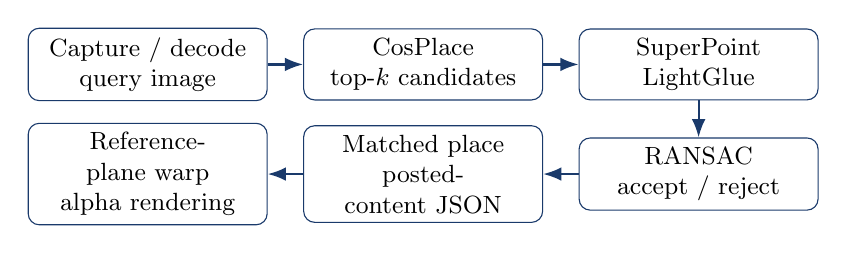
\begin{tikzpicture}[node distance=.47cm and .45cm,
 box/.style={draw=myblue,rounded corners,fill=white,align=center,text width=2.8cm,minimum height=.9cm,font=\small},
 arr/.style={-{Latex},thick,myblue}]
\node[box](q){Capture / decode\\query image};
\node[box,right=of q](g){CosPlace\\top-$k$ candidates};
\node[box,right=of g](l){SuperPoint\\LightGlue};
\node[box,below=of l](v){RANSAC\\accept / reject};
\node[box,left=of v](d){Matched place\\posted-content JSON};
\node[box,left=of d](r){Reference-plane warp\\alpha rendering};
\draw[arr](q)--(g);\draw[arr](g)--(l);\draw[arr](l)--(v);
\draw[arr](v)--(d);\draw[arr](d)--(r);
\end{tikzpicture}
\vspace{.35cm}
\begin{block}{Failure handling}
No accepted candidate $\Rightarrow$ no anchored post is rendered.
\end{block}
\SourceNote{Coarse-to-fine localisation principle: \cite{sarlin2019}; executed prototype uses planar verification.}
\end{frame}

\begin{frame}[t]{Geometry and Posted Content}
\begin{itemize}
\item Estimate a reference-to-query homography using tentative correspondences.
\item Check inlier count, inlier ratio and projective validity.
\item Retrieve content from the verified place record.
\item Use an explicit alpha mask; black asset pixels remain valid content.
\end{itemize}
\[
\widetilde{\mathbf x}_q\sim H_{r\rightarrow q}\widetilde{\mathbf x}_r,
\qquad H_{c\rightarrow q}=H_{r\rightarrow q}A_{c\rightarrow r}.
\]
\SourceNote{$A_{c\rightarrow r}$ maps asset corners to the stored reference polygon.}
\end{frame}

\section{Data and Experimental Protocol}
\begin{frame}[t]{Actual Evaluation Data}
\begin{itemize}
\item HPatches: \HpImages{} images, \HpPairs{} ground-truth homography pairs \cite{balntas2017}.
\item Tokyo: \TokyoImages{} real photographs from \TokyoSites{} selected sites \cite{torii2015}.
\item Synthetic stress test: \SyntheticQueries{} queries from six source images and three seeds.
\item Download manifests, CRC checks, SHA256 values and frozen protocols are retained.
\end{itemize}
\begin{alertblock}{Scope}
Tokyo is a custom cross-time query-to-query subset, not the official street-view retrieval benchmark.
\end{alertblock}
\end{frame}

\begin{frame}[t]{Real Day, Night and Sunset Images}
\centering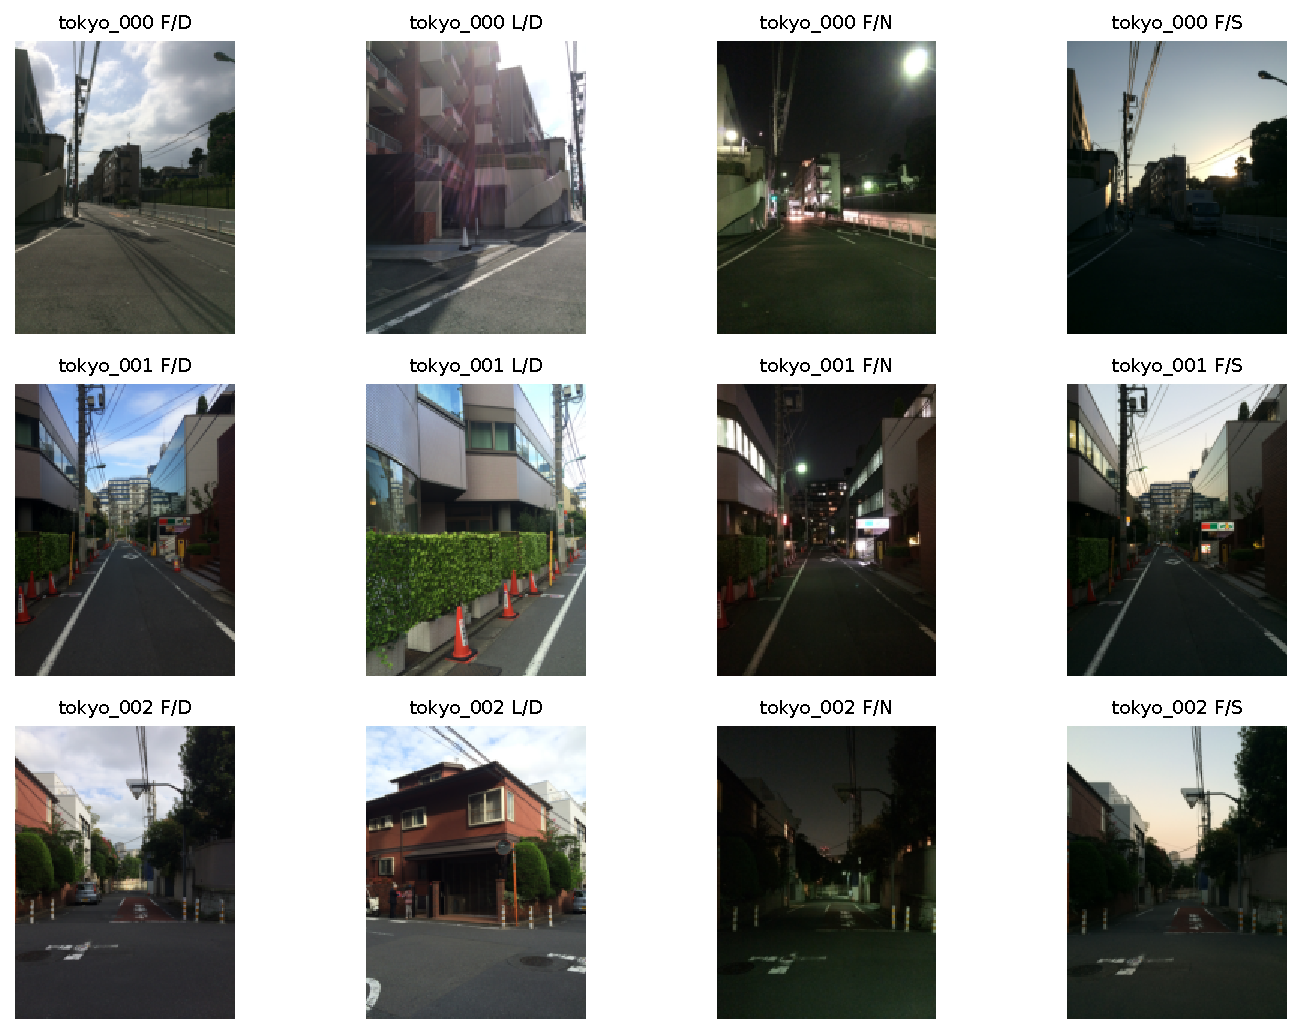
\includegraphics[width=\textwidth,height=5.8cm,keepaspectratio]{tokyo_contact.pdf}
\SourceNote{Actual downloaded Tokyo photographs. Front/day, left/day, front/night and front/sunset metadata define each retained site.}
\end{frame}

\begin{frame}[t]{Synthetic Appearance Stressors}
\centering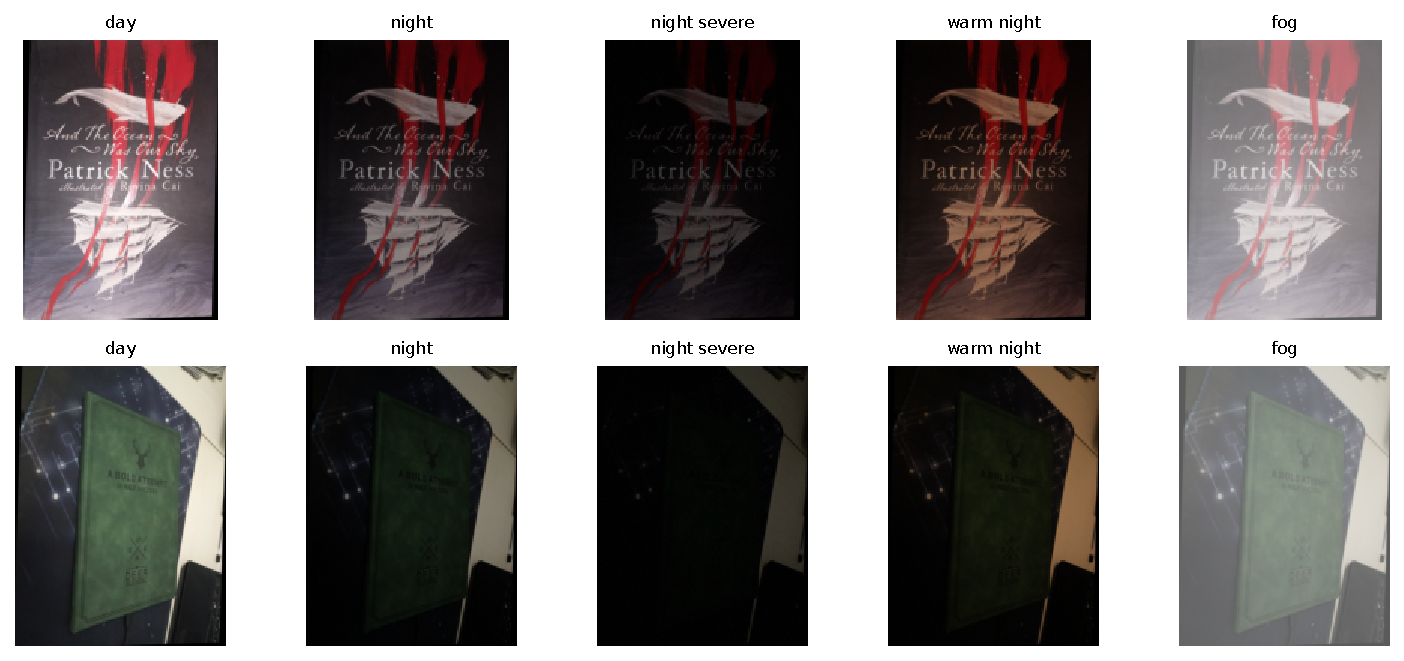
\includegraphics[width=\textwidth,height=5.5cm,keepaspectratio]{synthetic_contact.pdf}
\SourceNote{Executed gamma, gain, colour shift, noise and fog-like transformations; these are not real seasonal/weather observations.}
\end{frame}

\begin{frame}[t]{Experimental Controls and Metrics}
\small
\begin{itemize}
\item Same queries, reference galleries and geometric thresholds for A--D.
\item Maximum image side: 640 pixels; requested keypoints: 512.
\item RANSAC: 5-pixel threshold; acceptance: 12 inliers and 0.20 ratio.
\item Retrieval: Recall@1/5/10; decisions: correctly verified places.
\item HPatches/synthetic: accepted mean corner error $\leq5$ pixels.
\item Timing: isolated CPU queries with cached references; memory: process peak RSS.
\end{itemize}
\SourceNote{Host: Apple M2, 8 GB RAM, two CPU threads. No phone or calibrated metric-pose result is claimed.}
\end{frame}

\section{Results and Ablations}
\begin{frame}[t]{Local Matching: HPatches}
\centering
\small\MatchingTable
\vspace{.15cm}
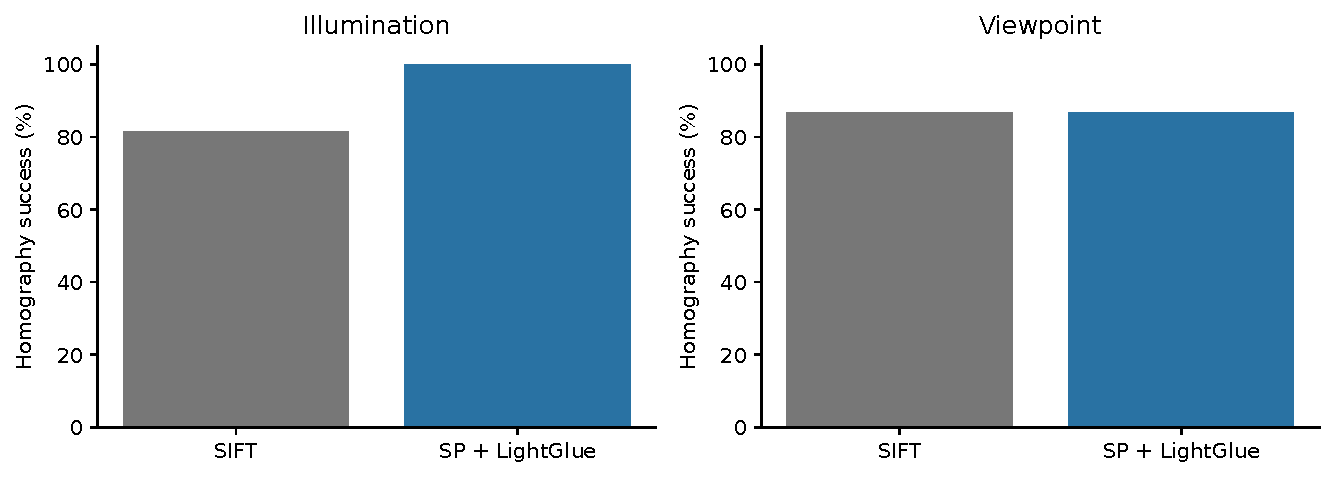
\includegraphics[width=.89\textwidth,height=3.65cm,keepaspectratio]{hpatches_success.pdf}
\SourceNote{Percent successful oracle-pair homographies. Learned matching improves this illumination subset; viewpoint success is tied.}
\end{frame}

\begin{frame}[t]{Tokyo Day-to-Night: Measured Results}
\centering\small\NightTable
\vspace{.25cm}
\begin{block}{Interpretation}
The full pipeline verifies \DayNightFullVerified\% of the selected queries. The gallery has only \TokyoSites{} sites and similar front-facing directions.
\end{block}
\SourceNote{Rates are percentages. Global retrieval alone does not produce an anchored transform.}
\end{frame}

\begin{frame}[t]{Viewpoint Change: A Negative Result}
\centering\small\ViewTable
\vspace{.25cm}
\begin{alertblock}{Global-shortlist limitation}
The full pipeline correctly verifies only \DayViewFullVerified\% when query direction changes. Exhaustive local search recovers some missed references.
\end{alertblock}
\SourceNote{Day-to-day means front-facing daytime reference to left-facing daytime query. It is not an unchanged-view control.}
\end{frame}

\begin{frame}[t]{Retrieval Across Real Tokyo Splits}
\centering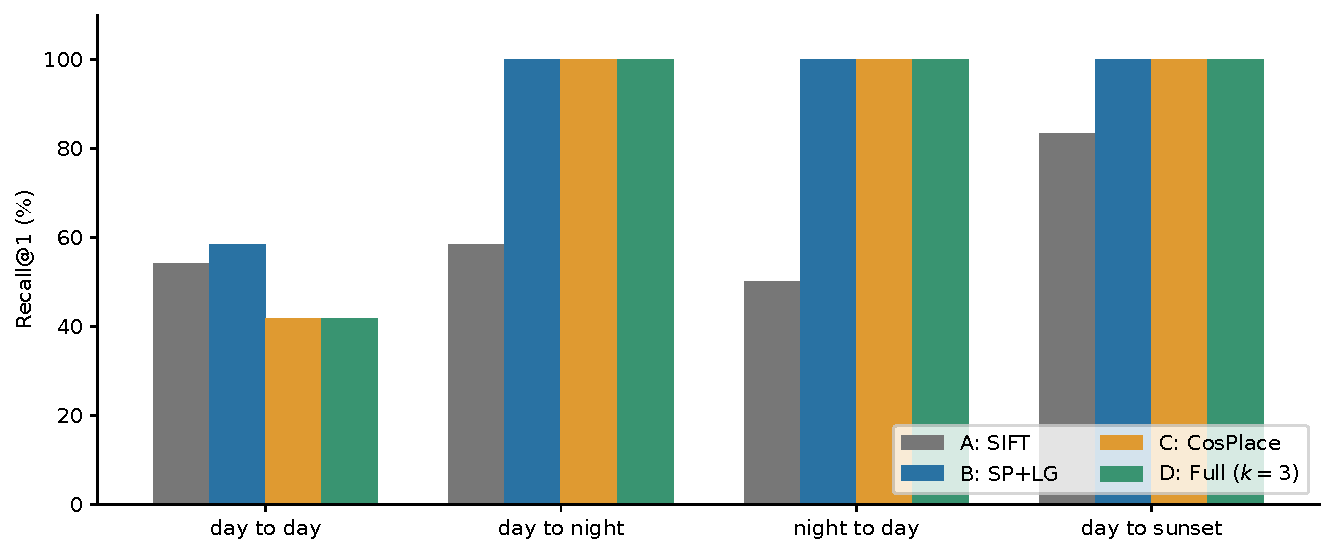
\includegraphics[width=\textwidth,height=5.7cm,keepaspectratio]{tokyo_retrieval.pdf}
\SourceNote{Actual Recall@1. Similar viewpoint across time can be easier than different viewpoint in daylight.}
\end{frame}

\begin{frame}[t]{Shortlist and Verification Ablations}
\centering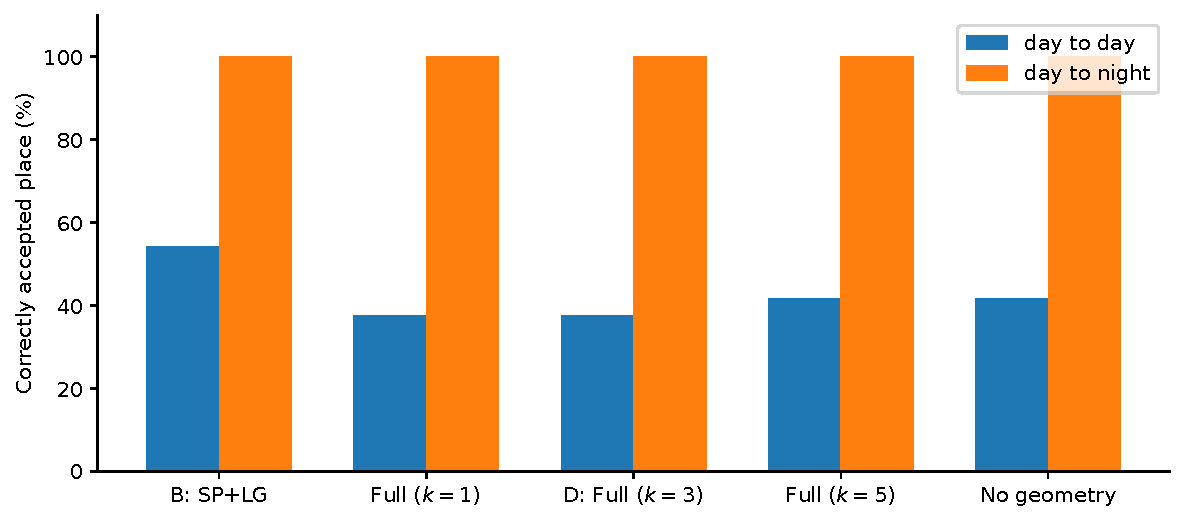
\includegraphics[width=\textwidth,height=5.3cm,keepaspectratio]{stage_ablation.pdf}
\SourceNote{Same queries: exhaustive learned search, $k=1/3/5$, and unverified top-result acceptance. More candidates can introduce competing hypotheses.}
\end{frame}

\begin{frame}[t]{Unknown Places and False Acceptance}
\centering\small\OpenSetTable
\vspace{.25cm}
\begin{alertblock}{Geometric support is not identity assurance}
Some unrelated queries still pass local verification. A production AR service needs stronger negative testing and calibrated decision policies.
\end{alertblock}
\SourceNote{Disjoint-collection diagnostic: HPatches queries against a Tokyo gallery; not a production false-positive bound.}
\end{frame}

\begin{frame}[t]{Short Adaptation: Three Fixed Seeds}
\centering\small\AdaptationTable
\vspace{.25cm}
\begin{itemize}
\item Frozen encoder; only a 512-to-128 linear projection is trained.
\item Eight training and sixteen held-out HPatches places; no Tokyo training.
\item With/without synthetic night augmentation; 120 steps per seed.
\item No consistent improvement over the pretrained descriptor.
\end{itemize}
\SourceNote{Mean Recall@1 (percent). The report includes seed standard deviations and intervals; compression and adaptation are not separated.}
\end{frame}

\begin{frame}[t]{Actual Correspondences Across Day/Night}
\centering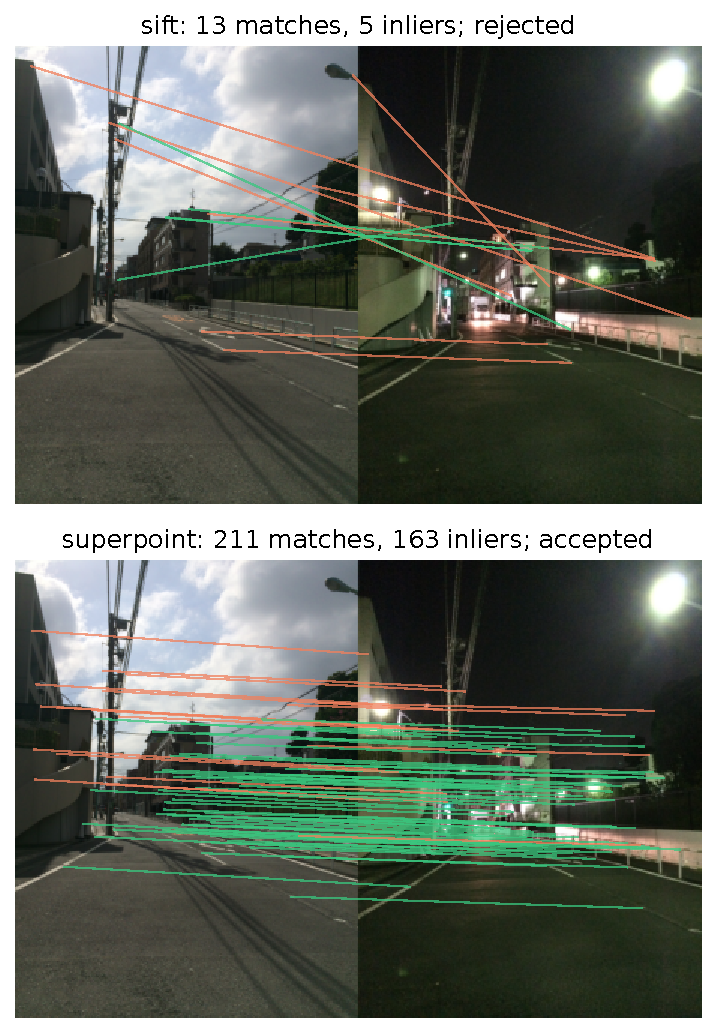
\includegraphics[width=\textwidth,height=5.8cm,keepaspectratio]{matches_tokyo_day_to_night.pdf}
\SourceNote{Recorded tentative matches: green denotes RANSAC inliers. Tokyo provides no independent homography or metric-pose ground truth here.}
\end{frame}

\begin{frame}[t]{Anchored-Content Comparison Demo}
\centering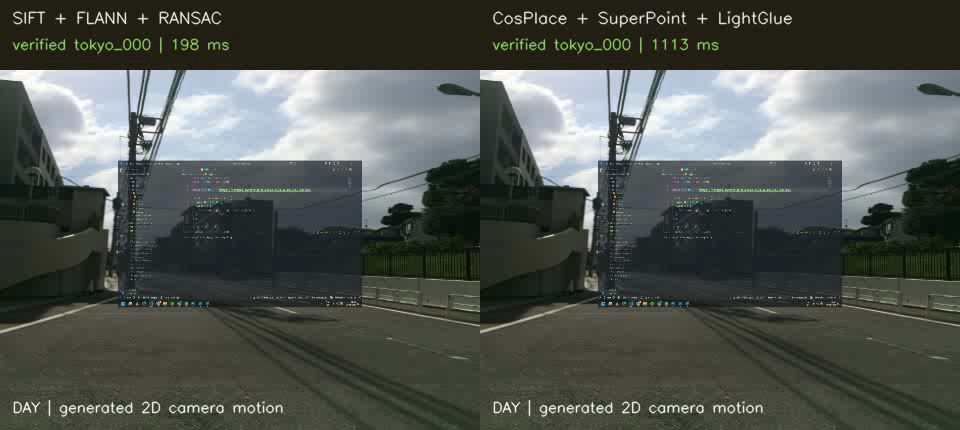
\includegraphics[width=\textwidth,height=5.35cm,keepaspectratio]{demo_frame.png}
\SourceNote{Actual classical/full executions. Real still images with labelled generated 2D camera motion; playback speed is not inference throughput.}
\end{frame}

\section{Deployment and Limitations}
\begin{frame}[t]{Measured CPU Latency and Memory}
\centering\small\RuntimeTable
\vspace{.20cm}
\begin{block}{Mobile implication}
Full-pipeline median: \LatencyFull{} ms per query on this CPU host. Use occasional recognition plus native tracking; this does not demonstrate phone real-time performance.
\end{block}
\SourceNote{Cached gallery; predecoded query; complete warm call and image-post rendering. Retrieval-only excludes geometry/rendering.}
\end{frame}

\begin{frame}[t]{Executed ONNX and INT8 Export}
\centering\small\QuantizationTable
\vspace{.25cm}
\begin{itemize}
\item Actual float ONNX parity and QDQ INT8 inference were tested.
\item Calibration uses reserved training places.
\item File size and descriptor latency improve; viewpoint accuracy decreases.
\item Export covers the global descriptor only.
\end{itemize}
\SourceNote{View R@1 is the Tokyo direction-change split. No full local-matcher, CoreML or phone export result is claimed.}
\end{frame}

\begin{frame}[t]{Limitations and Threats to Validity}
\begin{itemize}
\item Small selected galleries and repeated physical sites.
\item Synthetic night/fog cannot replace natural condition changes.
\item No calibrated 6-DoF map/pose accuracy or real seasonal benchmark.
\item Planar homography does not establish arbitrary 3D persistence.
\item CPU timings do not establish phone power, thermal or accelerator behaviour.
\end{itemize}
\end{frame}

\begin{frame}[t]{Ethics and a Persistent-AR Roadmap}
\begin{itemize}
\item Minimise camera and location retention; respect imagery terms.
\item Support consent, content visibility, reporting and deletion.
\item Add multi-direction references and real seasonal benchmarks.
\item Introduce calibrated maps/PnP and native AR tracking integration.
\item Validate wrong-place anchors and recovery on real devices.
\end{itemize}
\end{frame}

\section{Conclusions}
\begin{frame}[t]{Conclusions}
\begin{itemize}
\item Learned local matching improves the measured illumination subset.
\item Retrieval reduces learned search cost but can limit viewpoint recall.
\item Short adaptation does not consistently improve held-out retrieval.
\item Quantisation yields a concrete compact descriptor with an accuracy trade-off.
\item Reproducible code, measured results, report and demo are delivered.
\end{itemize}
\SourceNote{All numerical claims come from the retained Stitch experiment files. Full commands, seeds, hashes and failure analysis are in the report.}
\end{frame}

\section{References}
\begin{frame}[t]{References: Features and Retrieval}
\scriptsize
\begin{thebibliography}{99}
\bibitem{lowe2004} D. G. Lowe. Distinctive Image Features from Scale-Invariant Keypoints. \emph{IJCV}, 2004.
\bibitem{detone2018} D. DeTone, T. Malisiewicz and A. Rabinovich. SuperPoint: Self-Supervised Interest Point Detection and Description. \emph{CVPR Workshops}, 2018.
\bibitem{lindenberger2023} P. Lindenberger, P.-E. Sarlin and M. Pollefeys. LightGlue: Local Feature Matching at Light Speed. \emph{ICCV}, 2023.
\bibitem{berton2022} G. Berton, C. Masone and B. Caputo. Rethinking Visual Geo-Localization for Large-Scale Applications. \emph{CVPR}, 2022.
\end{thebibliography}
\end{frame}

\begin{frame}[t]{References: Benchmarks and Geometry}
\scriptsize
\begin{thebibliography}{99}
\bibitem[5]{balntas2017} V. Balntas, K. Lenc, A. Vedaldi and K. Mikolajczyk. HPatches: A Benchmark and Evaluation of Handcrafted and Learned Local Descriptors. \emph{CVPR}, 2017.
\bibitem[6]{torii2015} A. Torii, R. Arandjelovi\'c, J. Sivic, M. Okutomi and T. Pajdla. 24/7 Place Recognition by View Synthesis. \emph{CVPR}, 2015.
\bibitem[7]{sarlin2019} P.-E. Sarlin, C. Cadena, R. Siegwart and M. Dymczyk. From Coarse to Fine: Robust Hierarchical Localization at Large Scale. \emph{CVPR}, 2019.
\end{thebibliography}
\SourceNote{Complete verified bibliography and official source URLs accompany the report.}
\end{frame}

{\usebackgroundtemplate{
\includegraphics[width=\paperwidth,height=\paperheight]{white_bg.png}}
\begin{frame}[plain,c]
\begin{center}
{\Huge\bfseries\color{myblue} THANK YOU}\par\vspace{.5cm}
{\large\StudentName}\par\vspace{.2cm}
{\small\SchoolName}\par\vspace{.25cm}
{\normalsize Questions and Discussion}
\end{center}
\end{frame}}
\end{document}
